%\part*{Lezione 14/04/2020}
\paragraph{Qualche nota formale} Notiamo che l'espressione per $U_\ell$ in \eqref{0412_risUl} ha una forma che ricorda una lorentziana (come ci aspettavamo). \\
Poiché $E\sim E_R$ e la matrice $R$ non ha particolari discontinuità in $E$ ($R(E)\sim R(E_R)$\footnote{Non vale per $P_\ell$ che invece dipende fortemente dall'energia.}) si usa una forma approssimata per $\Gamma (E)$:
$$\frac{\Gamma (E)}{\Gamma (E_R)} \simeq \frac{P_\ell (E)}{P_\ell (E_R)}$$
Per cui definendo $\gamma^2 \equiv R_\ell (E_R)/ (S_\ell\, R_\ell)' (E_R)$ si ha $\Gamma (E) \simeq 2\gamma^2 P_\ell^2 (E)$.

\paragraph{Risonanza e autovalori} Un altro modo per vedere la risonanza è considerare $E\sim E_{\bar{n}\ell}$ con $\bar{n}$ fissato; infatti per tale energia $R$ diverge, per cui trascuriamo nella \eqref{0412_Rl3} tutti i termini con $n\not = \bar{n}$\footnote{Per semplicità da adesso in poi dal momento che non ci sarà ambiguità $\bar{n}\to n$}:
$$R_\ell (E) \simeq \frac{\gamma_{\bar{n}\ell}^2}{E_{\bar{n}\ell} - E}$$
Avremo allora per l'angolo di sfasamento in \eqref{0412_delta}:
$$\delta_\ell = \Phi_\ell + \tan^{-1} \PPc{\frac{P_\ell \gamma^2_{n\ell}}{E_{n\ell}-E - \gamma_{n\ell}^2 S_\ell(E)}}$$
Poiché vale anche \eqref{0412_risUl} si ha $\delta_\ell = \Phi_\ell + \tan^{-1} \ppc{\Gamma(E)/2(E_R-E)}$, da cui:
$$\Gamma (E) \simeq 2  \gamma^2_{n\ell}\,P_\ell (E)$$
\begin{equation}\label{0414_ERshift}
E_R \simeq E_{n\ell} - \gamma^2_{n\ell}\, S_\ell(E)
\end{equation}
Dunque, l'energia del polo di $R$ non corrisponde a quella di risonanza, ma questa è \textit{shiftata} di un certo fattore $\gamma^2_{n\ell} S_\ell(E)$\index{shift factor@\textit{shift factor}}\footnote{Da questo deriva appunto il nome \textit{shift factor}. Per quanto riguarda il \textit{penetration factor} esso dà informazioni sulla penetrazione della barriera coulombiana.}.

\subsection{Applicazioni}
Studiamo lo scattering $A_1+A_2$. La scelta delle $\varphi (r)$ è fondamentale per l'efficienza del metodo; in letteratura troviamo quelle per cui si ha la miglior convergenza:\index{metodo Rmatrix@metodo $R$-MATRIX!scelta delle funzioni d'onda}
\begin{align}
	-\;&\varphi_k (r) = \sin{\pp{[}{\frac{\pi r}{a}\ppc{k-\frac{1}{2}}}{]}}%
	\label{0414_funz1} \\
	-\;&\varphi_k (r) = r^{\ell+1} \exp{\ppc{-\frac{r^2}{b^2_k}}}\quad \text{con } b_k = b_1 x_0^{k-1}%
	\label{0414_funz2} \\
	-\;&\varphi_k (r) = (-1)^{N+i} \ppc{\frac{r}{ax_k}}^n \sqrt{a x_k (1-x_k)} \frac{P_N(2r/a - 1)}{r-ax_k} \quad \text{con } x_k \: : \: P_N(2x_k - 1) = 0 %
	\label{0414_funz3}
\end{align}
Per tutte $a$ corrisponde al solito \textit{channel radius}\index{channel radius@\textit{channel radius}}, mentre $b_1$ e $x_0$ nelle \eqref{0414_funz2} sono parametri da determinare.
Le ultime, \eqref{0414_funz3}, sono dette funzioni di Lagrange\index{funzioni di Lagrange}, i $P_N$ sono i polinomi di Legendre\index{polinomi di Legendre} e gli $x_k$ i loro zeri; l'esponente $n$ viene spesso preso $n\sim 1$.\\
Passiamo adesso alla trattazione di 2 esempi di scattering:
\begin{enumerate}
	\item $p+\ce{^{12}C}$: dati $V_N+V_C$ e $\varphi_i$ si ricava $\delta_\ell$ e si cerca la risonanza a $E_R = 0.42$ MeV e una larghezza (risonanza stretta) $\Gamma=37$ keV come \textit{test}.
	\item $\alpha + \alpha$: procendendo come per il caso precedente si cerca $E_R= (11.35 \pm 0.15)$ MeV e una larghezza (risonanza larga) $\Gamma\simeq 3.5$ MeV.\\
	\texttt{[NON RIPORTATO]}  
\end{enumerate}

\paragraph{Esempio ${p+\ce{^{12}C}}$} Riportiamo i risultati per lo sfasamento in Figura \ref{0414_p12C} e per la funzione d'onda ridotta di onda $S$ in Figura \ref{0414_p12C-2}. In generale si osserva che le funzioni di Lagrange hanno convergenza più veloce e un miglior accordo tra regione esterna e interna per $u_0$.
\begin{figure}[h]
	\centering
	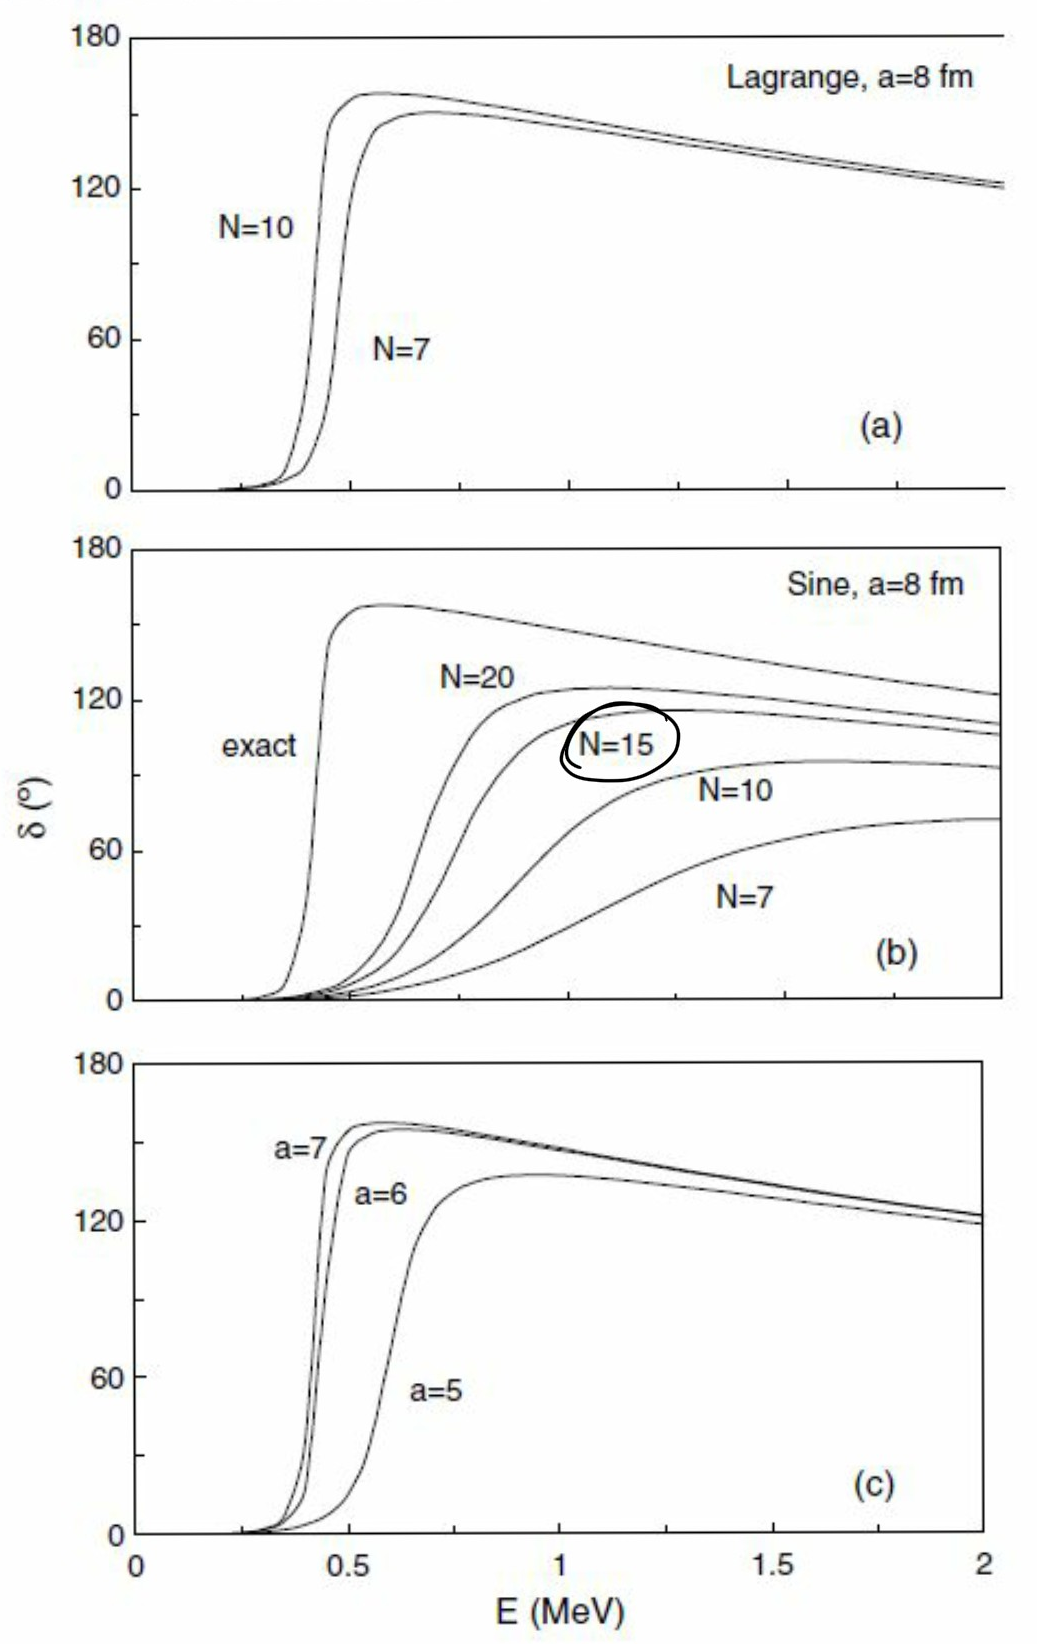
\includegraphics[scale=0.2]{Immagini/0414_metodi.png}
	\caption{Risultati per lo sfasamento di $p+\ce{^{12}C}$: (a) funzioni di Lagrange con $a=8$ fm, notiamo che già per $N=10$ si ha quasi la convergenza; (b) funzioni seno con $a=8$ fm, la convergenza è più lenta (non basta $N=20$); (c) convergenza delle funzioni seno in funzione di $a$, il risultato è $a=7$.}
	%!! Lei dice così ma a me non torna molto che siano le funzioni seno
	\label{0414_p12C}
\end{figure}
\begin{figure}[h]
	\centering
	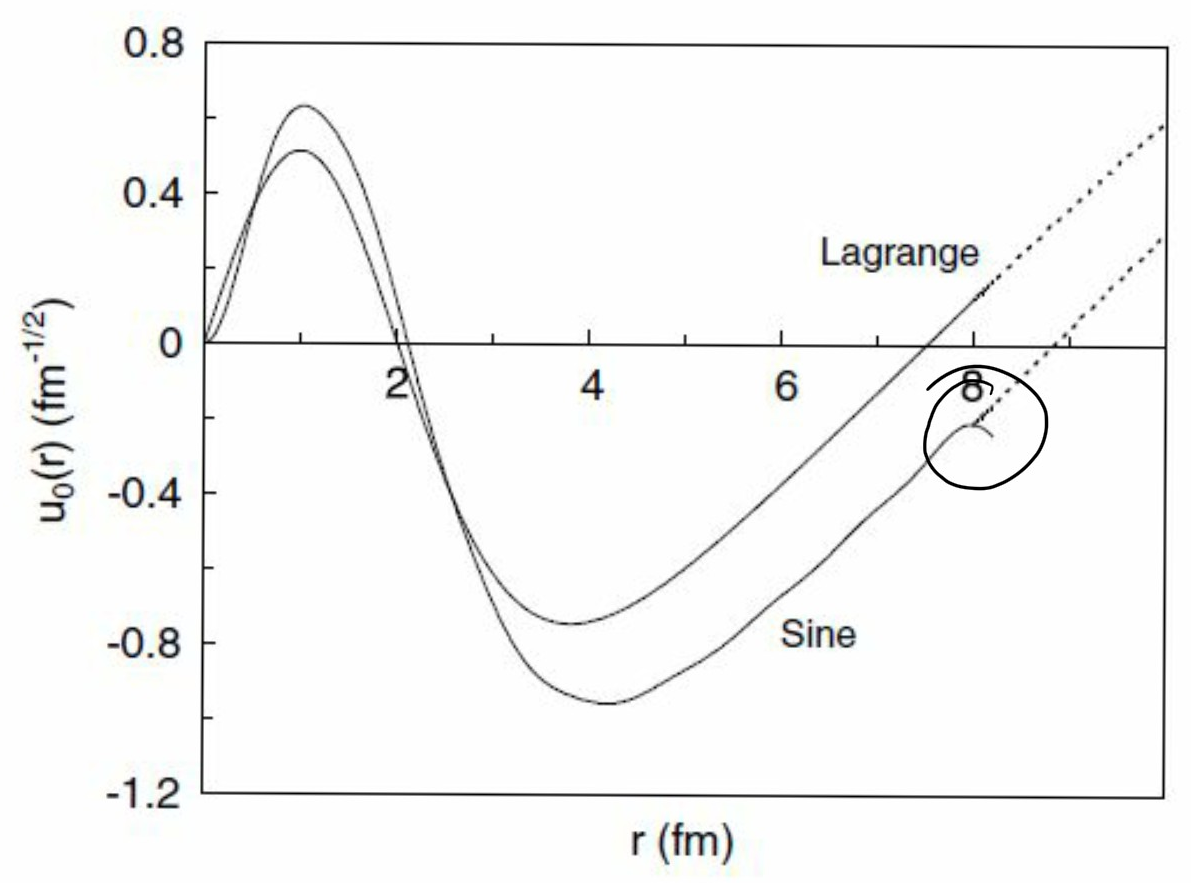
\includegraphics[scale=0.2]{Immagini/0414_metodi2.png}
	\caption{Funzioni d'onda ridotte calcolate per $\ell=0,N=15$ e $a=8$ fm con le funzioni di Lagrange e con quelle seno. Notiamo che quest'ultime portano a funzioni \vir{sporche} nella zona di raccordo con l'esterno.}
	\label{0414_p12C-2}
\end{figure}
\noindent In Figura \ref{0414_p12C-3} è invece riportato il \textit{matching} dei parametri che permette di stimare la bontà della convergenza. Le funzioni seno sono le prime a essere state studiate, ma come mostrano i risultati le gaussiane e quelle di Lagrange sono migliori.
%%%% ? Qui definisce un certo \epsilon ma sinceramente non capisco a cosa serva dal momemento che non compare nella tabella
\begin{figure}[h]
	\centering
	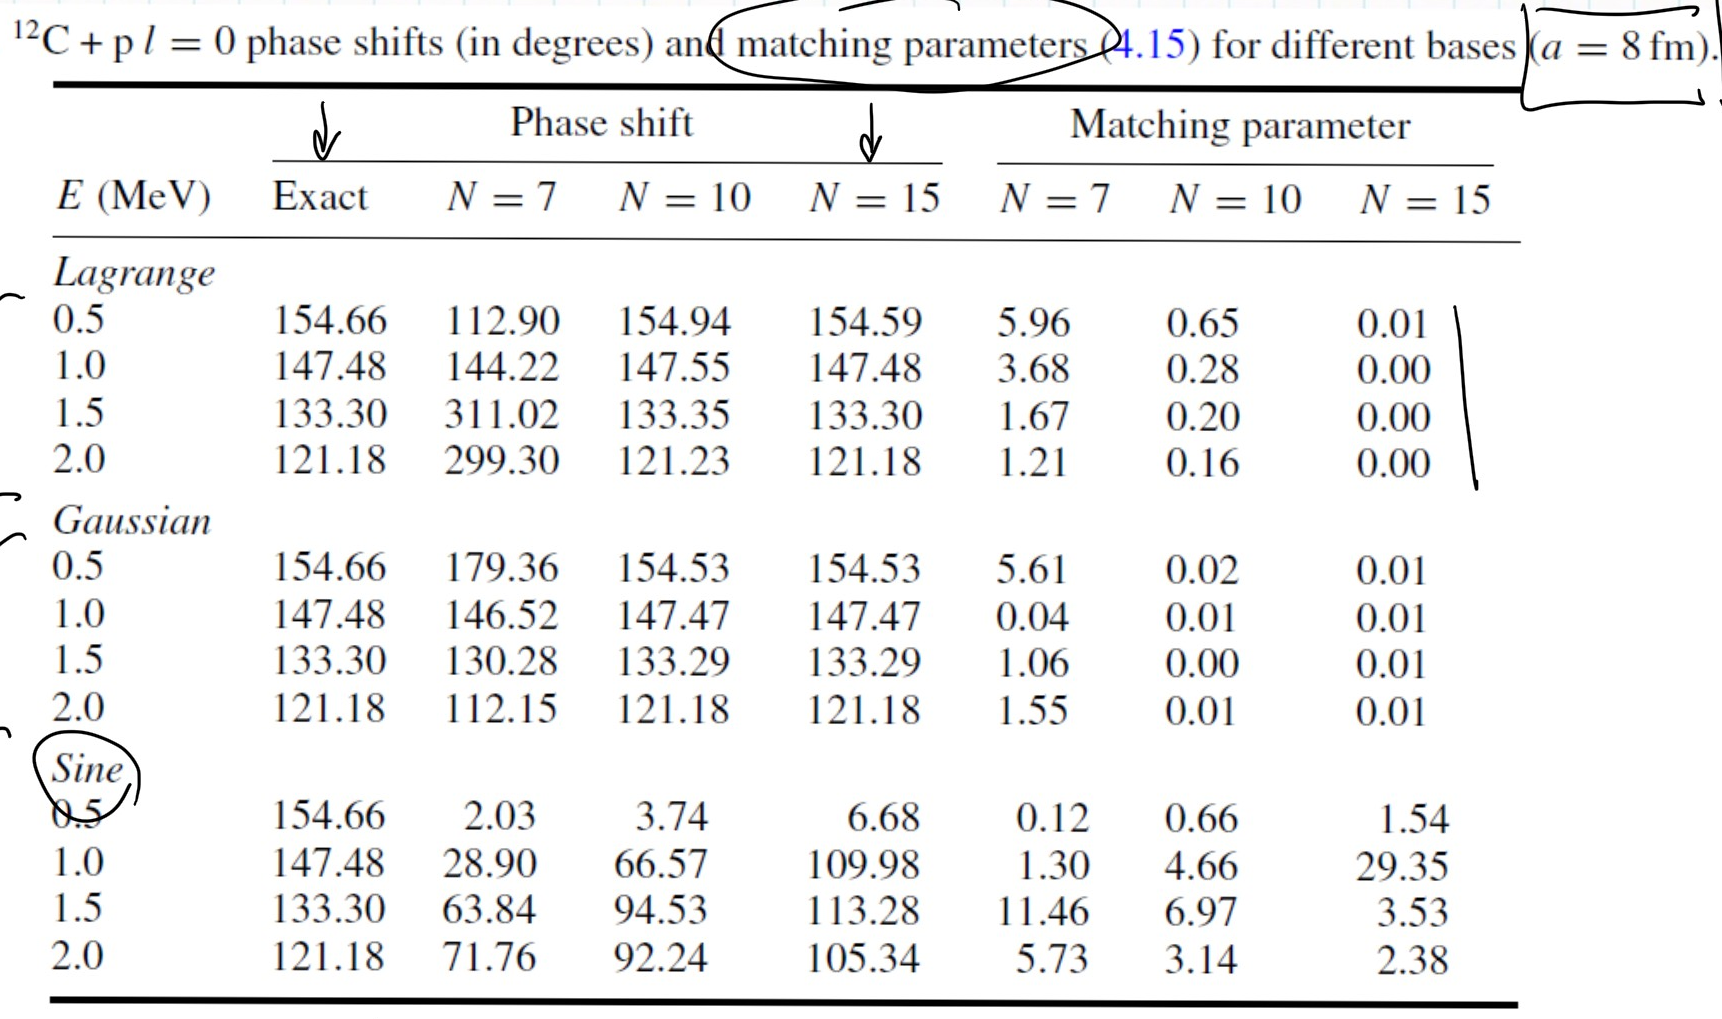
\includegraphics[scale=0.2]{Immagini/0414_metodi3.png}
	\caption{\textit{Matching} dei parametri per $a=8$.}
	\label{0414_p12C-3}
\end{figure}

\subparagraph{Una piccola osservazione} Notiamo la differenza con un metodo \textit{ab-initio}\index{metodo ab-initio@metodo \textit{ab-initio}}: non abbiamo fatto uno studio su 13 nucleoni, ma abbiamo lavorato solo con 2 oggetti $p$ e $\ce{^{12}C}$.

\newpage

\section{Phenomenological RM}
Riprendiamo l'espressione che avevamo trovato per $\delta$ nel caso di risonanza:
$$\delta_\ell = \Phi_\ell + \tan^{-1} {\ppc{\frac{\Gamma_R /2}{E_R-E}}}$$
con $\Gamma_R\equiv 2\gamma^2 \, P_\ell(E_R)$. Se quindi abbiamo dati sperimentali di $\Gamma_R$ ed $E_R$ avremo un certo $\gamma^2_{obs}$, per cui possiamo ricavare l'andamento in funzione dell'energia di $\delta_\ell$ e $u^{int}$ e di conseguenza dal formalismo sviluppato finora anche $\sigma(E)$ e $S(E)$ per ogni energia. In sintesi è questo il metodo \textit{ph}RM\index{metodo Rmatrix@metodo $R$-MATRIX!Phenomenological}.

\paragraph{Un metodo semplice} Dobbiamo fare attenzione perché $E_{n\ell}$ e $\gamma_{n\ell}$ (come abbiamo già visto) non corrispondono a $E_R$ e $\gamma_{obs}$. Per ricavare la relazione tra queste quantità come in \eqref{0414_ERshift} non possiamo seguire gli stessi passaggi fatti in precedenza (altrimenti $\gamma_{n\ell} \sim \gamma_{obs}$), ma il risultato sarà simile. Consideriamo per semplicità un solo polo per $R(E)$ in $E_1$ e sviluppiamo $S_\ell$ intorno a questo valore:
$$S_\ell(E) = S_\ell(E_1) + (E-E_1) S_\ell'(E_1)$$
Allora per $\delta_\ell$ si avrà\footnote{Si omette il pedice $_\ell$.}:
\begin{align*}
	\delta &\simeq \Phi + \tan^{-1}{\ppc{\frac{\gamma_1^2 \, P(E)}{E_1 - E - \gamma^2_1 \, S(E_1)-\gamma^2_1 \, (E-E_1) \, S'(E_1)}}} = \\
	&= \Phi + \tan^{-1}{\ppc{\frac{\gamma_1^2 \, P(E)}{E_1 - \gamma^2_1 \, S(E_1)+\gamma^2_1 \, E_1 \, S'(E_1) - E \, (1+\gamma^2_1 \, S'(E_1))}}} = \\
	&= \Phi + \tan^{-1}{\ppc{\underbrace{\frac{\gamma_1^2}{1+\gamma^2_1 S'(E_1)}}_{\gamma^2_{obs}} P(E) \, \frac{1}{\underbrace{E_1 - \gamma_1 \, S(E_1)/(1+\gamma_1^2\, S'(E_1))}_{E_R} - E}}} = \\
	&= \Phi + \tan^{-1}{\ppc{\frac{\gamma^2_{obs}\, P(E_R)}{E_R - E}}}
\end{align*}
Da cui si ottiene\footnote{Rimettiamo il pedice.}:
\begin{align}
	&\gamma_{1\ell}^2 \simeq \frac{\gamma_{obs}^2}{1-\gamma_{obs}^2\, S_{\ell}'(E_R)} \label{0414_gamma1} \\
	&E_{1\ell} \simeq E_R + \gamma^2_{1\ell} \, S_\ell (E_R) \label{0414_E1}
\end{align}
Da queste si ottiene $R_\ell(E)$ e quindi $\sigma(E)$ o $S(E)$.

\paragraph{Il caso di $p + \ce{^{12}C}$}
In letteratura si definiscono spesso queste quantità:
\begin{align*}
	&\gamma_W \equiv \frac{3\hbar^2}{2\mu a} \\
	&\theta_{obs}^2 \equiv \frac{\gamma^2_{obs}}{\gamma_W^2} \\
	&\theta_{1}^2 \equiv \frac{\gamma^2_{1}}{\gamma_W^2}
\end{align*}
Quando $\theta\sim 1$ i nuclei che collidono conservano la loro struttura nella risonanza.
%? \footnote{\acc{E} infatti possibile osservare $p$ e $\ce{^{12}C}$ nella risonanza di $\ce{^{13}N}$.}
%! Questo non torna tanto perché il \theta di quello non è 1, ci si avvicina di più \ce{^{12}C} + \alpha \to \ce{^{15}N} + p (sempre che non sia la reazione con l'ossigeno)
Riportiamo in Figura \ref{0414_phRM1} i risultati per tale reazione di scattering in funzione di $a$, dal momento che $P_\ell$ ne dipende e quindi di conseguenza anche $\Gamma_R$. In Figura \ref{0414_phRM2} invece è riportato l'andamento ottenuto per il fattore astrofisico. Anche se il calcolo sembra riprodurre bene i dati, si è considerato il $\ce{^{12}C}$ puntiforme, ma osserviamo che questa è un'approssimazione dal momento che nel risultato $\theta\not = 1$.
\begin{figure}[h]
	\centering
	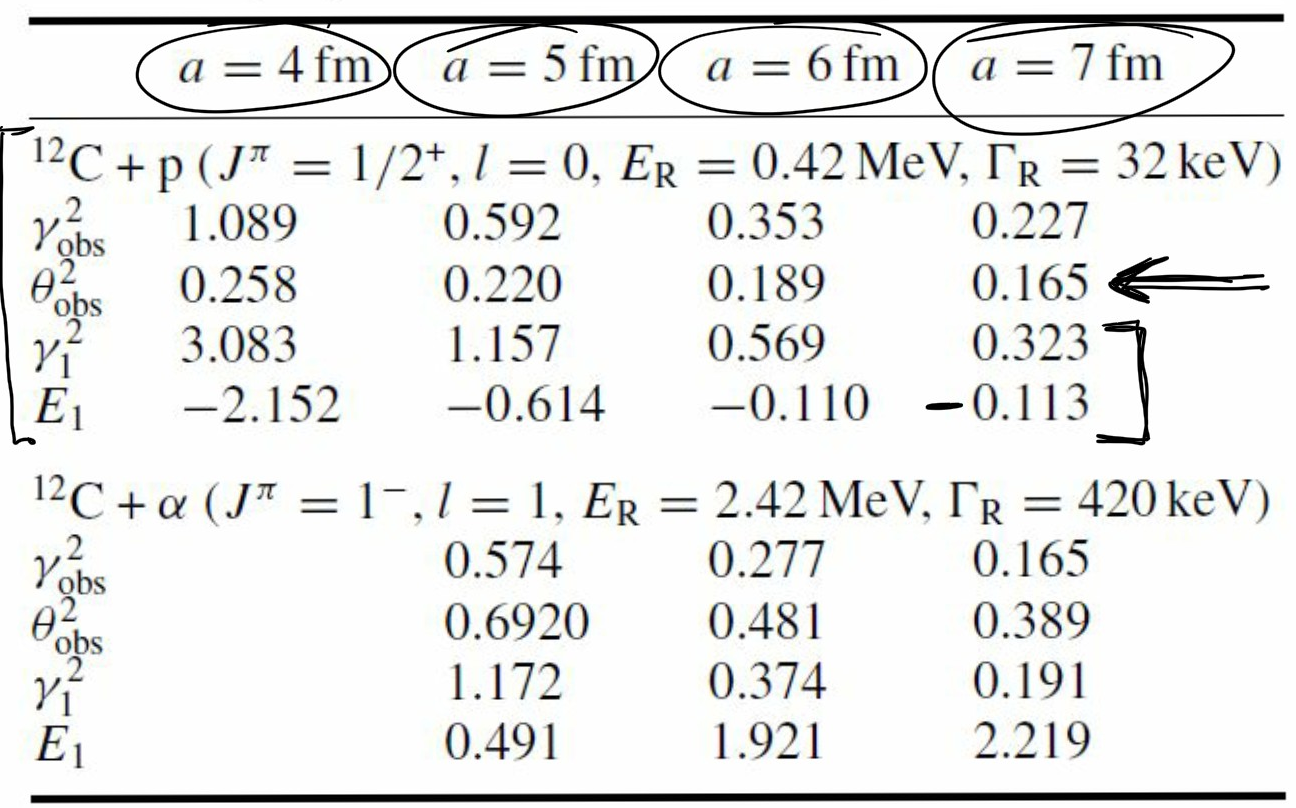
\includegraphics[scale=0.3]{Immagini/0414_RM.png}
	\caption{Risultati per lo scattering $p + \ce{^{12}C}$.}
	\label{0414_phRM1}
\end{figure}
\\
\noindent \acc{E} possibile rendersi conto di questa approssimazione perché l'andamento di $S(E)$ (e quindi anche della sezione d'urto) dev'essere riscalato rispetto a quello dei dati; si introduce allora un termine di correzione $\mathcal{S}$ (\textit{overall factor}) detto \textbf{fattore spettroscopico}\index{fattore spettroscopico}\footnote{Tecnicamente per ottenere un'espressione di questo parametro avrei bisogno di un metodo \textit{ab-initio}, ma se lo avessi non ci sarebbe motivo di usare il metodo RM.} che moltiplica il fattore astrofisico. Nel caso particolare da noi studiato per ottenere accordo\footnote{Per decidere l'accordo si cerca di fare un \textit{matching} per il picco della risonanza.} $\mathcal{S} = 0.45$ (come in Figura \ref{0414_phRM2}).
\begin{figure}[h]
	\centering
	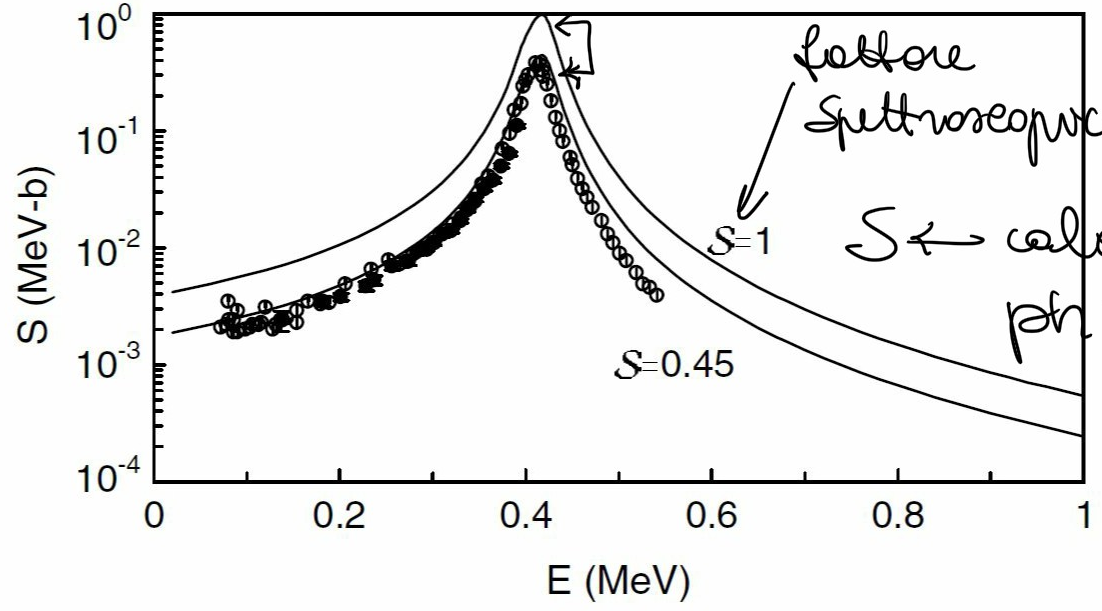
\includegraphics[scale=0.3]{Immagini/0414_RM2.png}
	\caption{Andamento del fattore astrofisico ricavato con il metodo \textit{ph}RM. La curva continua in alto è l'andamento calcolato senza correzione, mentre quella che \vir{fitta} i dati corrisponde a un fattore spettroscopico pari a 0.45.}
	\label{0414_phRM2}
\end{figure}
\newpage
\paragraph{Conclusioni} Concludiamo così la trattazione dei metodi di studio di reazioni. I metodi \text{ab-initio}\index{metodo ab-initio@metodo \textit{ab-initio}} sono certamente indipendenti dai dati, ma molto dispendiosi e complicati; il metodo RM\index{metodo Rmatrix@metodo $R$-MATRIX} invece permette il calcolo anche nel caso di molti nucleoni, ma dipende fortemente dai dati a disposizione (in un certo senso è un fit). 



\chapter{Tecniche sperimentali di misura}
Studieremo in questo capitolo alcuni degli esperimenti condotti per misure di reazioni nucleari di interesse astrofisico.
\paragraph{Tecniche di misura} 
Abbiamo visto che la sezione d'urto \vir{precipita} vari ordini di grandezza per energie sempre più piccole, quindi vi saranno pochissimi eventi; non solo a quelle energie l'ordine di grandezza del segnale è circa lo stesso di quello del fondo, per cui si deve trovare una soluzione che permetta di migliorare la misura. Esistono principalmente due strategie:
\begin{enumerate}
	\item Metodi diretti di misura con l'uso di qualche \vir{trucco}.
	\item Metodi indiretti di misura.
\end{enumerate}

\section{Metodi diretti}
Innanzitutto per risolvere il problema del numero di eventi si utilizzano acceleratori ad altissima luminosità (fasci molto densi). Per quanto riguarda il \textit{background}, si cerca di schermalo il più possibile: i Laboratori Nazionali del Gran Sasso (LNGS)\footnote{Link al sito: \url{https://www.lngs.infn.it/it/astrofisica-nucleare}}\index{Laboratori Nazionali del Gran Sasso} sono usati per esperimenti con pochi eventi, come quelli di fisica nucleare (LUNA), sui neutrini (decadimento $0\nu\beta\beta$\footnote{Si tratta di un decadimento $\beta\beta$ nel quale non dovrebbe comparire il neutrino, ma se così non fosse allora $\nu=\bar{\nu}$.} o lo stesso Borexino\esperimento{Borexino}) e sulla \textit{dark matter} (XENON1T\esperimento{XENON1T} o DARKSIDE\esperimento{DARKSIDE}).
%\\ Cerchiamo però di capire quali siano i tipi di \textit{background} e come schermarli.

\paragraph{Raggi cosmici}\index{ZZBackground@\textbf{Background}!raggi cosmici}
Particelle cariche (muoni per esempio) ad alta energia molto penetranti. Per schermare questo tipo di fondo esistono principalmente due tipi di tecniche:
\begin{itemize}
	\item \textit{active shielding}\index{active shielding@\textit{active shielding}}: si circonda il rivelatore con uno secondario sensibile ai raggi cosmici e si studiano gli eventi in anticoincidenza.
	\item \textit{passive shielding}\index{passive shielding@\textit{passive shielding}}: si posizione il rivelatore in un mezzo schermante (come un blocco o il sottosuolo), tuttavia si può incorrere nel problema di un aumento nel rumore dovuto all'interazione tra il mezzo schermante e i raggi.
\end{itemize}
L'unità di misura dello schermaggio è \textit{l'acqua equivalente}\index{acqua equivalente}; al Gran Sasso per esempio vi sono 1400 m di roccia che corrispondo a 3800 m di acqua equivalente e questo comporta una riduzione per muoni dell'ordine di $\ord{6}$, per neutroni di $\ord{3}$ e per raggi $\gamma$ di $10$.\\
In Figura \ref{0414_bckgamma} riportiamo lo spettro dei raggi $\gamma$ in grigio sulla superficie e in nero nei laboratori del Gran Sasso.
Fino a circa 3 MeV si ha un certo flusso di fotoni dovuto per una \vir{piccola} parte ai raggi cosmici (schermati) e per il contributo maggiore agli elementi radioattivi presenti nelle rocce; per energie superiori a 2.6 MeV invece abbiamo principalemente raggi cosmici, che vengono appunto ben schermati ( fatta eccezione per alcuni picchi di reazioni note e quindi semplici da contare).\\
Ci chiediamo adesso se sia possibile migliorare lo schermaggio. La soluzione più semplice sembrerebbe quella di aggiungere un ulteriore schermo, per esempio circondando il rivelatore di piombo, ed effettivamente questo si fa, come mostrato in Figura \ref{0414_bckgamma} (b). Tuttavia, il mezzo dev'essere \vir{ripulito} da qualsiasi impurità radioattiva e spesso quel che si fa è aspettare un tempo sufficiente affinché divenga inerte.\\ 
Un piccolo aneddoto a tal riguardo: nel Gennaio del 2016 in Sardegna fu ritrovata sul fondo del mare una nave romana che conteneva 30 lingotti di piombo; non avevano alcun valore artistico o economico, ma per i fisici furono \vir{oro} dal momento che la concentrazione di isotopi radioattivi al suo interno dopo 2000 anni era effimera e per questa ragione furono portati nei LNGS, dove tuttora si trovano.\complementi{Piombo romano nei LNGS}

\begin{figure}[!h]
	\centering
	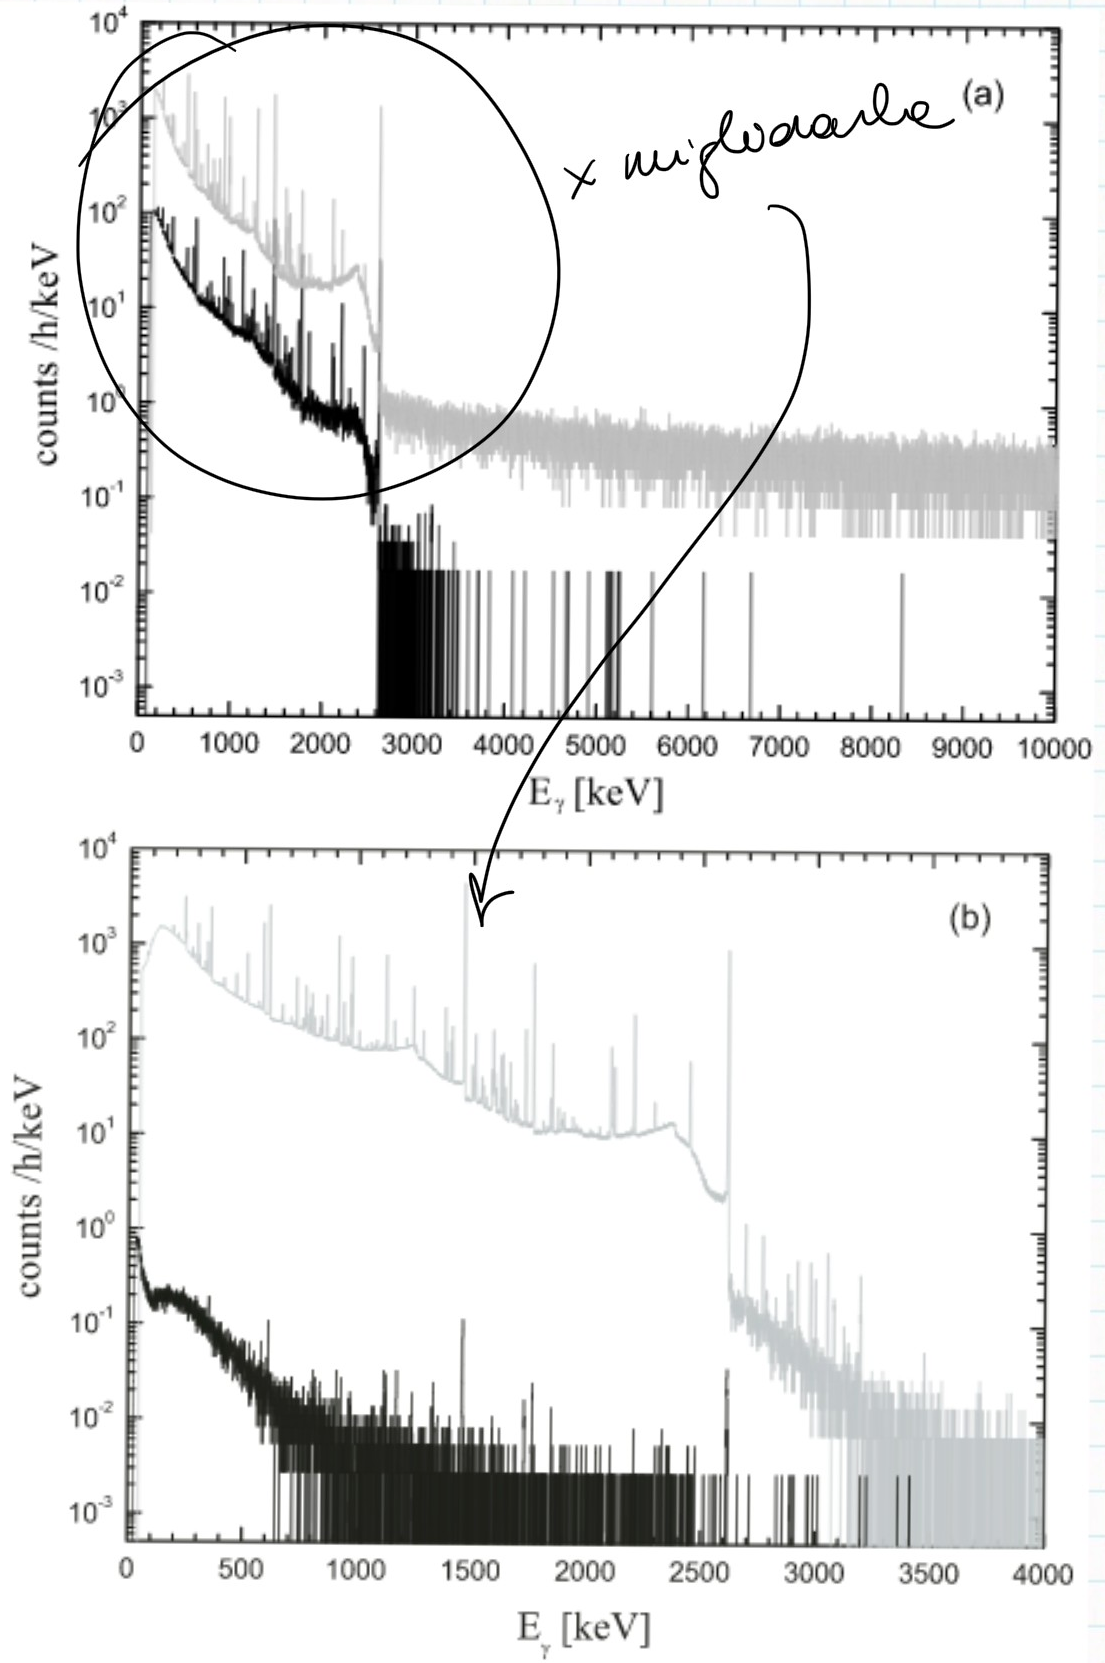
\includegraphics[scale=0.3]{Immagini/0414_background.png}
	\caption{Spettro dei raggi $\gamma$ sulla superfice in grigio e nei laboratori in nero: il grafico (a) riporta i dati senza altro schermaggio, il grafico (b) invece mostra i dati con uno schermo aggiuntivo.}
	\label{0414_bckgamma}
\end{figure}

\paragraph{Un nemico nel sottosuolo}\index{ZZBackground@\textbf{Background}!radon} 
Abbiamo visto che porsi nel sottosuolo permette lo schermaggio dai raggi $\gamma$, tuttavia si presenta un'altra difficoltà: il radon $\ce{^{222}Rn}$. Questo è radioattivo e si trova in stato gassoso, intrappolato nel sottosuolo circola nella zona sperimentale. Per risolvere tale problema tipicamente si installa il rivelatore in un contenitore in cui si genera un flusso d'aria continuo.